\documentclass[9pt, apectratio=43,unicode]{beamer}
\usetheme{Moscow}

\usepackage[utf8]{inputenc}
\usepackage[T2A]{fontenc}
\usepackage[main=russian,english]{babel}

\usepackage{amsmath,amssymb}

\renewcommand{\thefootnote}{\fnsymbol{footnote}}
\hypersetup{pdfauthor={Paul Ostanin}}

%\usepackage{concmath}
%\usepackage{euler}

\usepackage{mathtools}

\graphicspath{ {images/} }

\title[Двумерная модель земной ионосферы]{Двумерная модель земной ионосферы}
\author[Останин П. А.]{Останин Павел Антонович \\ \vspace{1ex} Научный руководитель: Кулямин Дмитрий Вячеславович}
\date{}

\newcommand{\colorhref}[2]{\href{#1}{\textcolor{miptbase!30!black}{#2}}}

\begin{document}

\begin{frame}[plain]
\titlepage
\end{frame}

\def\L{\mathcal{L}}

\section{Постановка задачи}
\begin{frame}\frametitle{Постановка задачи}
Основные задачи:
\begin{itemize}
\item[•] Построение динамической трёхмерной модели Земной ионосферы;
\item[•] Согласование с уже разработанной моделью нейтральной термосферы ИВМ РАН.
\end{itemize}

Уравнение, описывающее эволюцию ионной концентрации: $$\dfrac{\partial n_i}{\partial t} = -div(n_i \vec{u}_\parallel)-div\left(n_i\dfrac{1}{B^2}[\vec{E}\times \vec{B}] \right)+$$ $$+div\left(D\left[\nabla_\parallel n_i +n_i\dfrac{1}{T_p}\nabla_\parallel T_p - \dfrac{n_i m_i}{2kT_p}\vec{g}_\parallel\right]\right)+[P-k_in_i].$$

\end{frame}

\begin{frame}\frametitle{Уравнение в сферических координатах в приближении тонкого сферического слоя}

$$\dfrac{\partial n_i}{\partial t} = DYZ(n_i)+DTr(n_i)+Tr(n_i)+[P-kn_i].$$

$$Tr(n_i) = \dfrac{1}{a\cos\varphi}\dfrac{\partial}{\partial\lambda}\left[n_i\dfrac{1}{B}(E_y\sin I + E_z\cos I)\right]+\dfrac{1}{a\cos\varphi}\dfrac{\partial}{\partial\varphi}\bigg[\bigg(u_z\sin I \cos I - u_y\cos^2 I -$$ $$- \dfrac{E_x}{B}\sin I\bigg)n_i\cos\varphi\bigg]+\dfrac{\partial}{\partial z}\left[\left(u_y\cos I \sin I -u_z\sin^2 I - \dfrac{E_x}{B}\cos I\right)n_i\right];$$

$$DYZ(n_i) = \dfrac{1}{a\cos\varphi}\dfrac{\partial}{\partial\varphi}\left(D\cos\varphi\left[\dfrac{1}{a}\dfrac{\partial n_i}{\partial\varphi} \cos^2 I -\dfrac{\partial n_i}{\partial z}\cos I\sin I\right]\right)+ \dfrac{\partial}{\partial z}\bigg(D\bigg[\dfrac{\partial n_i}{\partial z}\sin^2 I -$$ $$- \dfrac{1}{a}\dfrac{\partial n_i}{\partial\varphi}\cos I \sin I\bigg]\bigg);$$ 

$$DTr(n_i) = \dfrac{1}{a\cos\varphi}\dfrac{\partial}{\partial \varphi}\bigg[\bigg(\dfrac{1}{a}\dfrac{1}{T_p}\dfrac{\partial T_p}{\partial\varphi}\cos^2 I-\dfrac{1}{T_p}\dfrac{\partial T_p}{\partial z}\cos I \sin I - \dfrac{1}{H}\sin I \cos I\bigg)Dn_i\cos\varphi\bigg] +$$ $$+ \dfrac{\partial}{\partial z}\bigg[\bigg(-\dfrac{1}{a}\dfrac{1}{T_p}\dfrac{\partial T_p}{\partial \varphi}\cos I \sin I +\dfrac{1}{T_p}\dfrac{\partial T_p}{\partial z}\sin^2 I+\dfrac{1}{H}\sin^2I\bigg)Dn_i\bigg].$$
\end{frame}


\section{Численное моделирование}

\subsection{Метод расщепления}

\begin{frame}\frametitle{Метод расщепления}
\begin{itemize}
\item[•] На первом шаге расщепления решается уравнение для $z$-диффузии в проекции со смешанной производной:

$$\dfrac{\partial n}{\partial t} =P-kn+\dfrac{\partial}{\partial z}\biggl[D\sin^2 I\left(\dfrac{\partial n}{\partial z}+\left(\dfrac{1}{T_p}\dfrac{\partial T_p}{\partial z}+\dfrac{1}{H}\right)n\right)-$$ $$-\dfrac{1}{a}D\sin I\cos I\left(\dfrac{\partial n}{\partial\varphi}+\dfrac{1}{T_p}\dfrac{\partial T_p}{\partial\varphi}n\right)\biggr];$$
 
\item[•] На втором шаге добавляется диффузия по $y$:
 
 $$\dfrac{\partial n}{\partial t} = \dfrac{1}{a\cos\varphi} \dfrac{\partial }{\partial \varphi}\left[\dfrac{D}{a}\cdot(\cos^2  I \cos\varphi)\cdot\dfrac{\partial n}{\partial \varphi} - u\cdot(\sin I \cos I \cos\varphi)\cdot n \right]=$$$$=  \dfrac{1}{\cos\varphi} \dfrac{\partial }{\partial \varphi}\left[\dfrac{D}{a^2}A(\varphi)\dfrac{\partial n}{\partial \varphi} - \dfrac{u}{2a}B(\varphi) n \right];$$

\item[•] На третьем шаге добавляется перенос $Tr(n_i)$.
\end{itemize}

\end{frame}


\subsection{Используемые разностные схемы}
\begin{frame}\frametitle{Используемые разностные схемы}
\begin{itemize}
\item[•] Для аппроксимации диффузионых слагаемых используется схема $$\dfrac{\partial}{\partial z}D\dfrac{\partial n}{\partial z} \approx \dfrac{1}{h_{i+1/2}}\left(\dfrac{D_{i+1/2}(n_{i+1}-n_i)}{h_i}-\dfrac{D_{i-1/2}(n_{i}-n_{i-1})}{h_{i-1}}\right);$$

\item[•] Слагаемые, отвечающие переносу $\dfrac{\partial}{\partial z}(u n)$ с эффективной скоростью $u$ аппроксимируются центральной разностью;

\smallskip

\parbox[b][5cm][t]{50mm}{
\item[•] Аппроксимация смешанной производной $\dfrac{\partial}{\partial\varphi}\left(B(\varphi)\dfrac{\partial n}{\partial z}\right)$ со вторым порядком осуществляется направленными разностями в зависимости от знака $B(\varphi)$.
}
\hfill
\parbox[b][5cm][t]{60mm}{
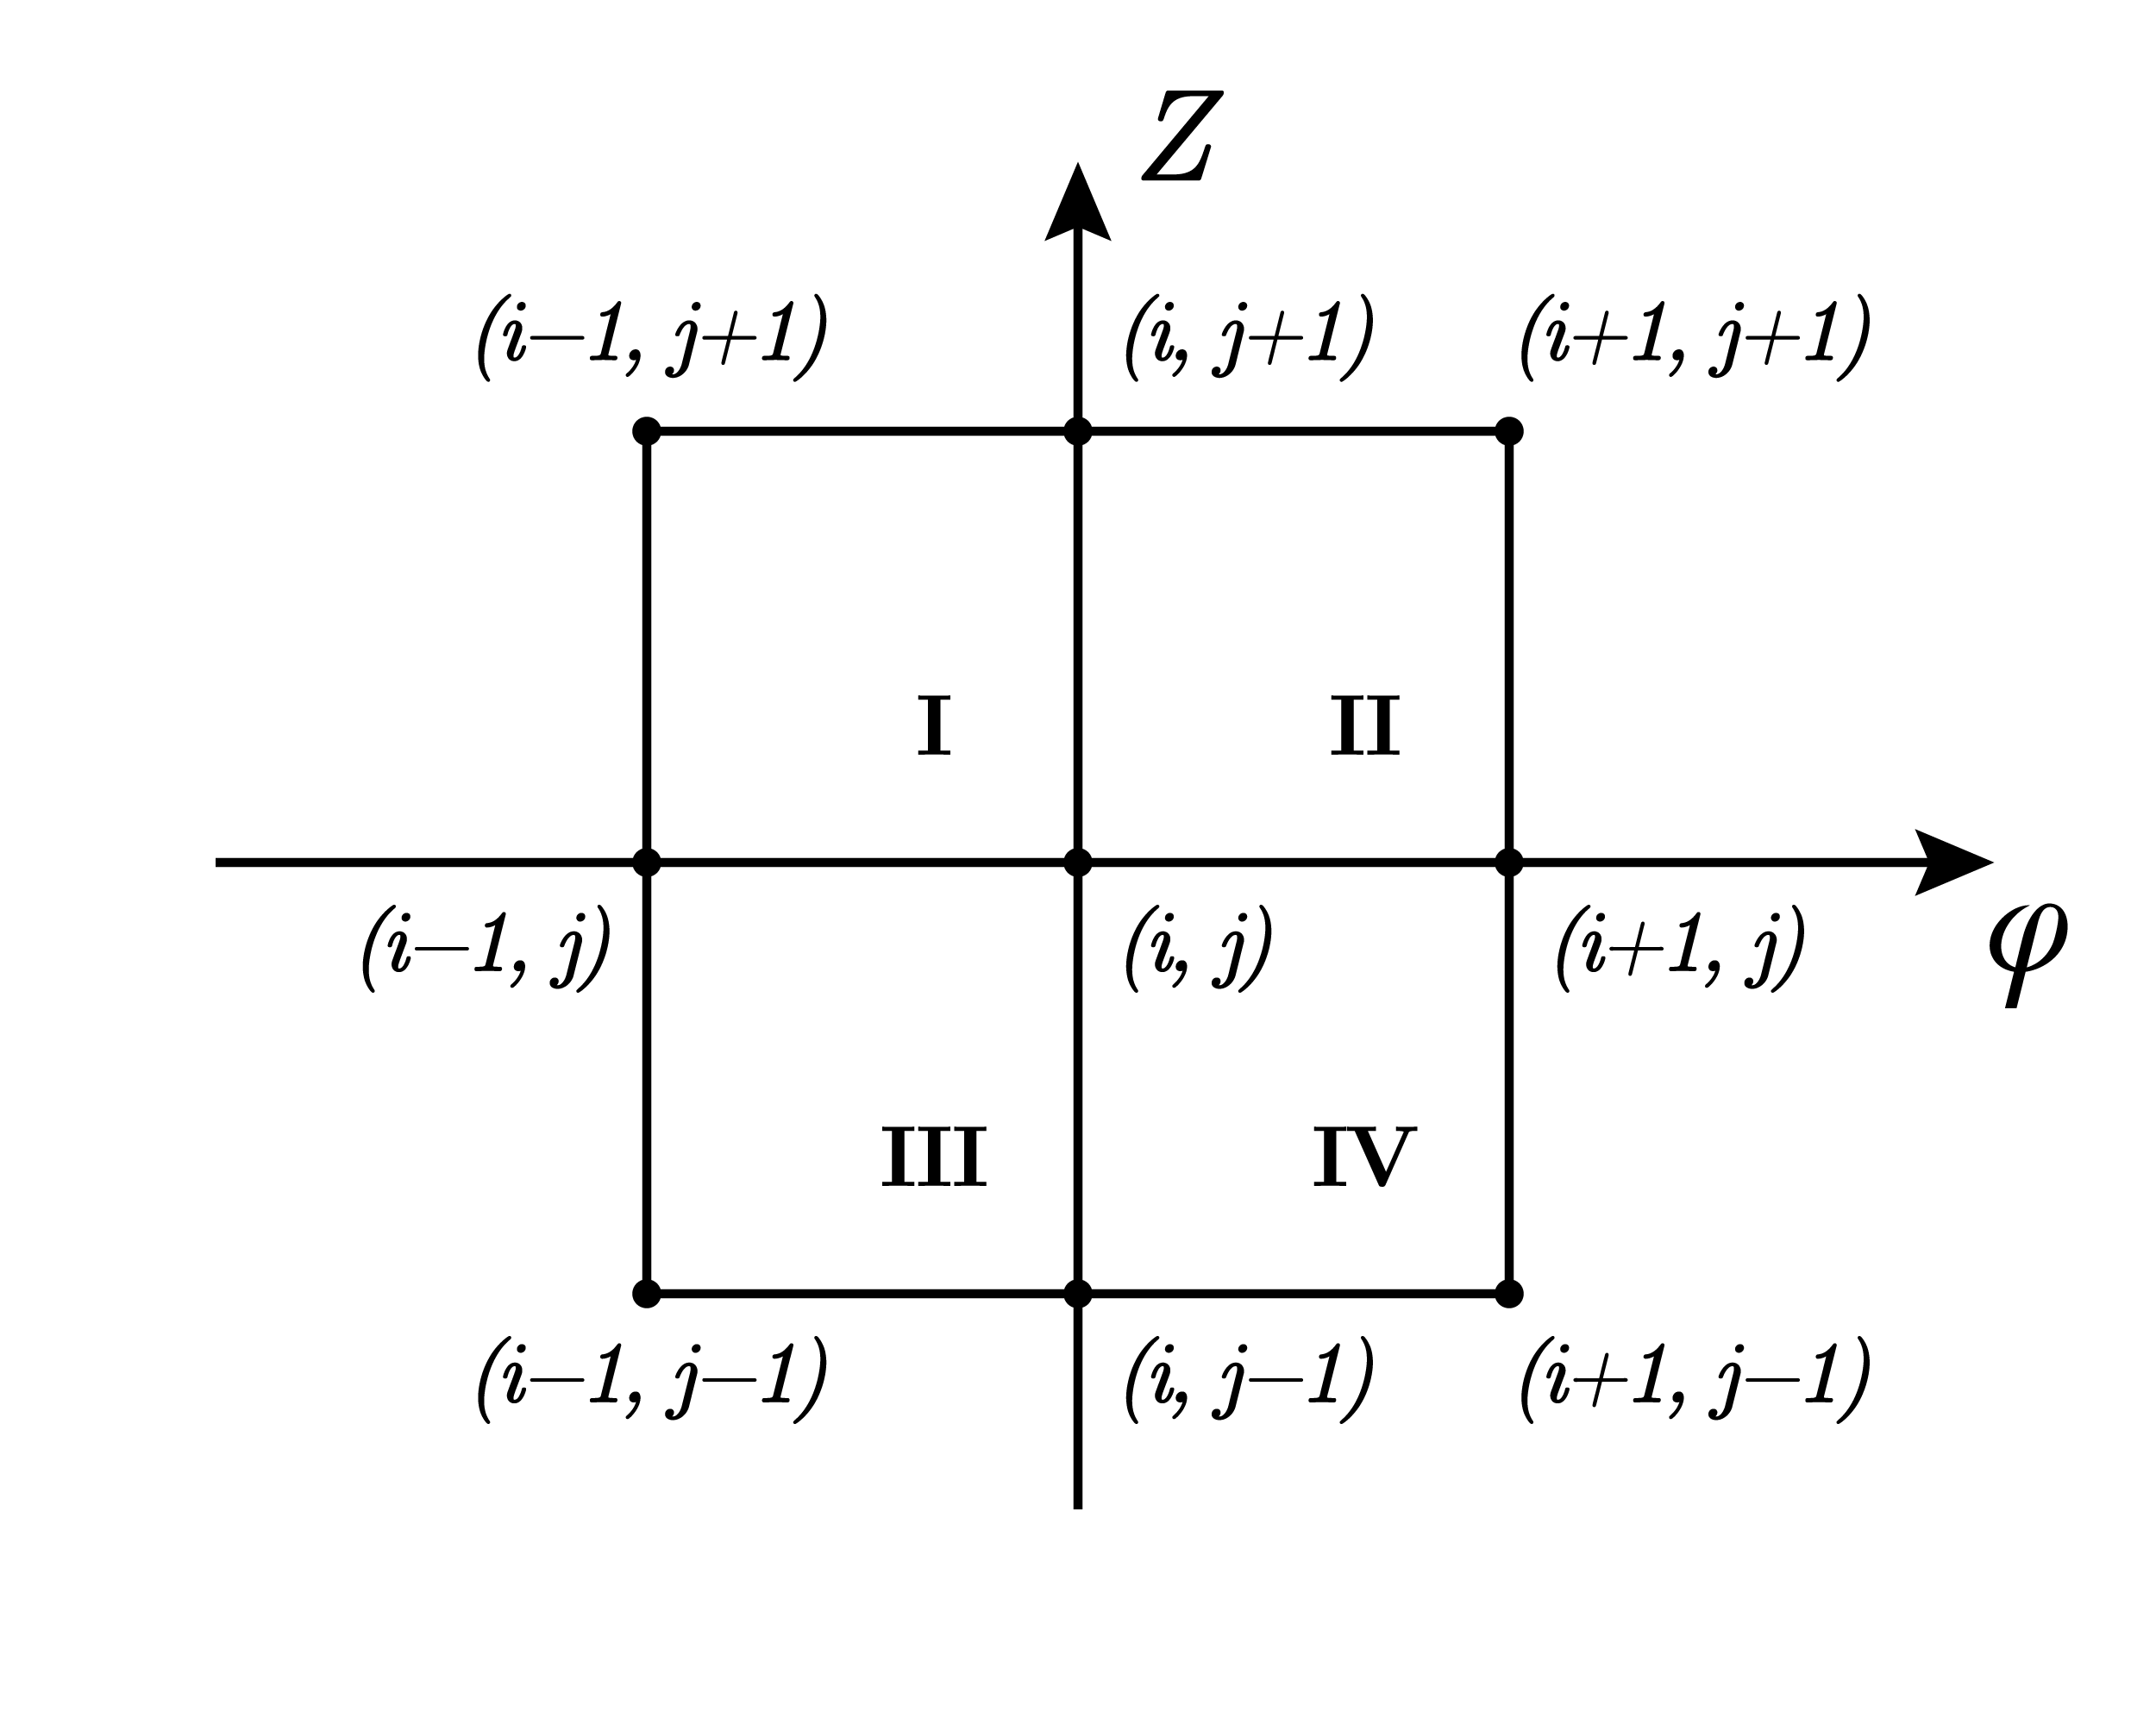
\includegraphics[scale = 0.3]{square}
}

\end{itemize}
\end{frame}


\subsection{Околополюсные точки и потеря порядка аппроксимации}
\begin{frame}\frametitle{Околополюсные точки и потеря порядка аппроксимации}



\parbox[b][5cm][t]{40mm}{
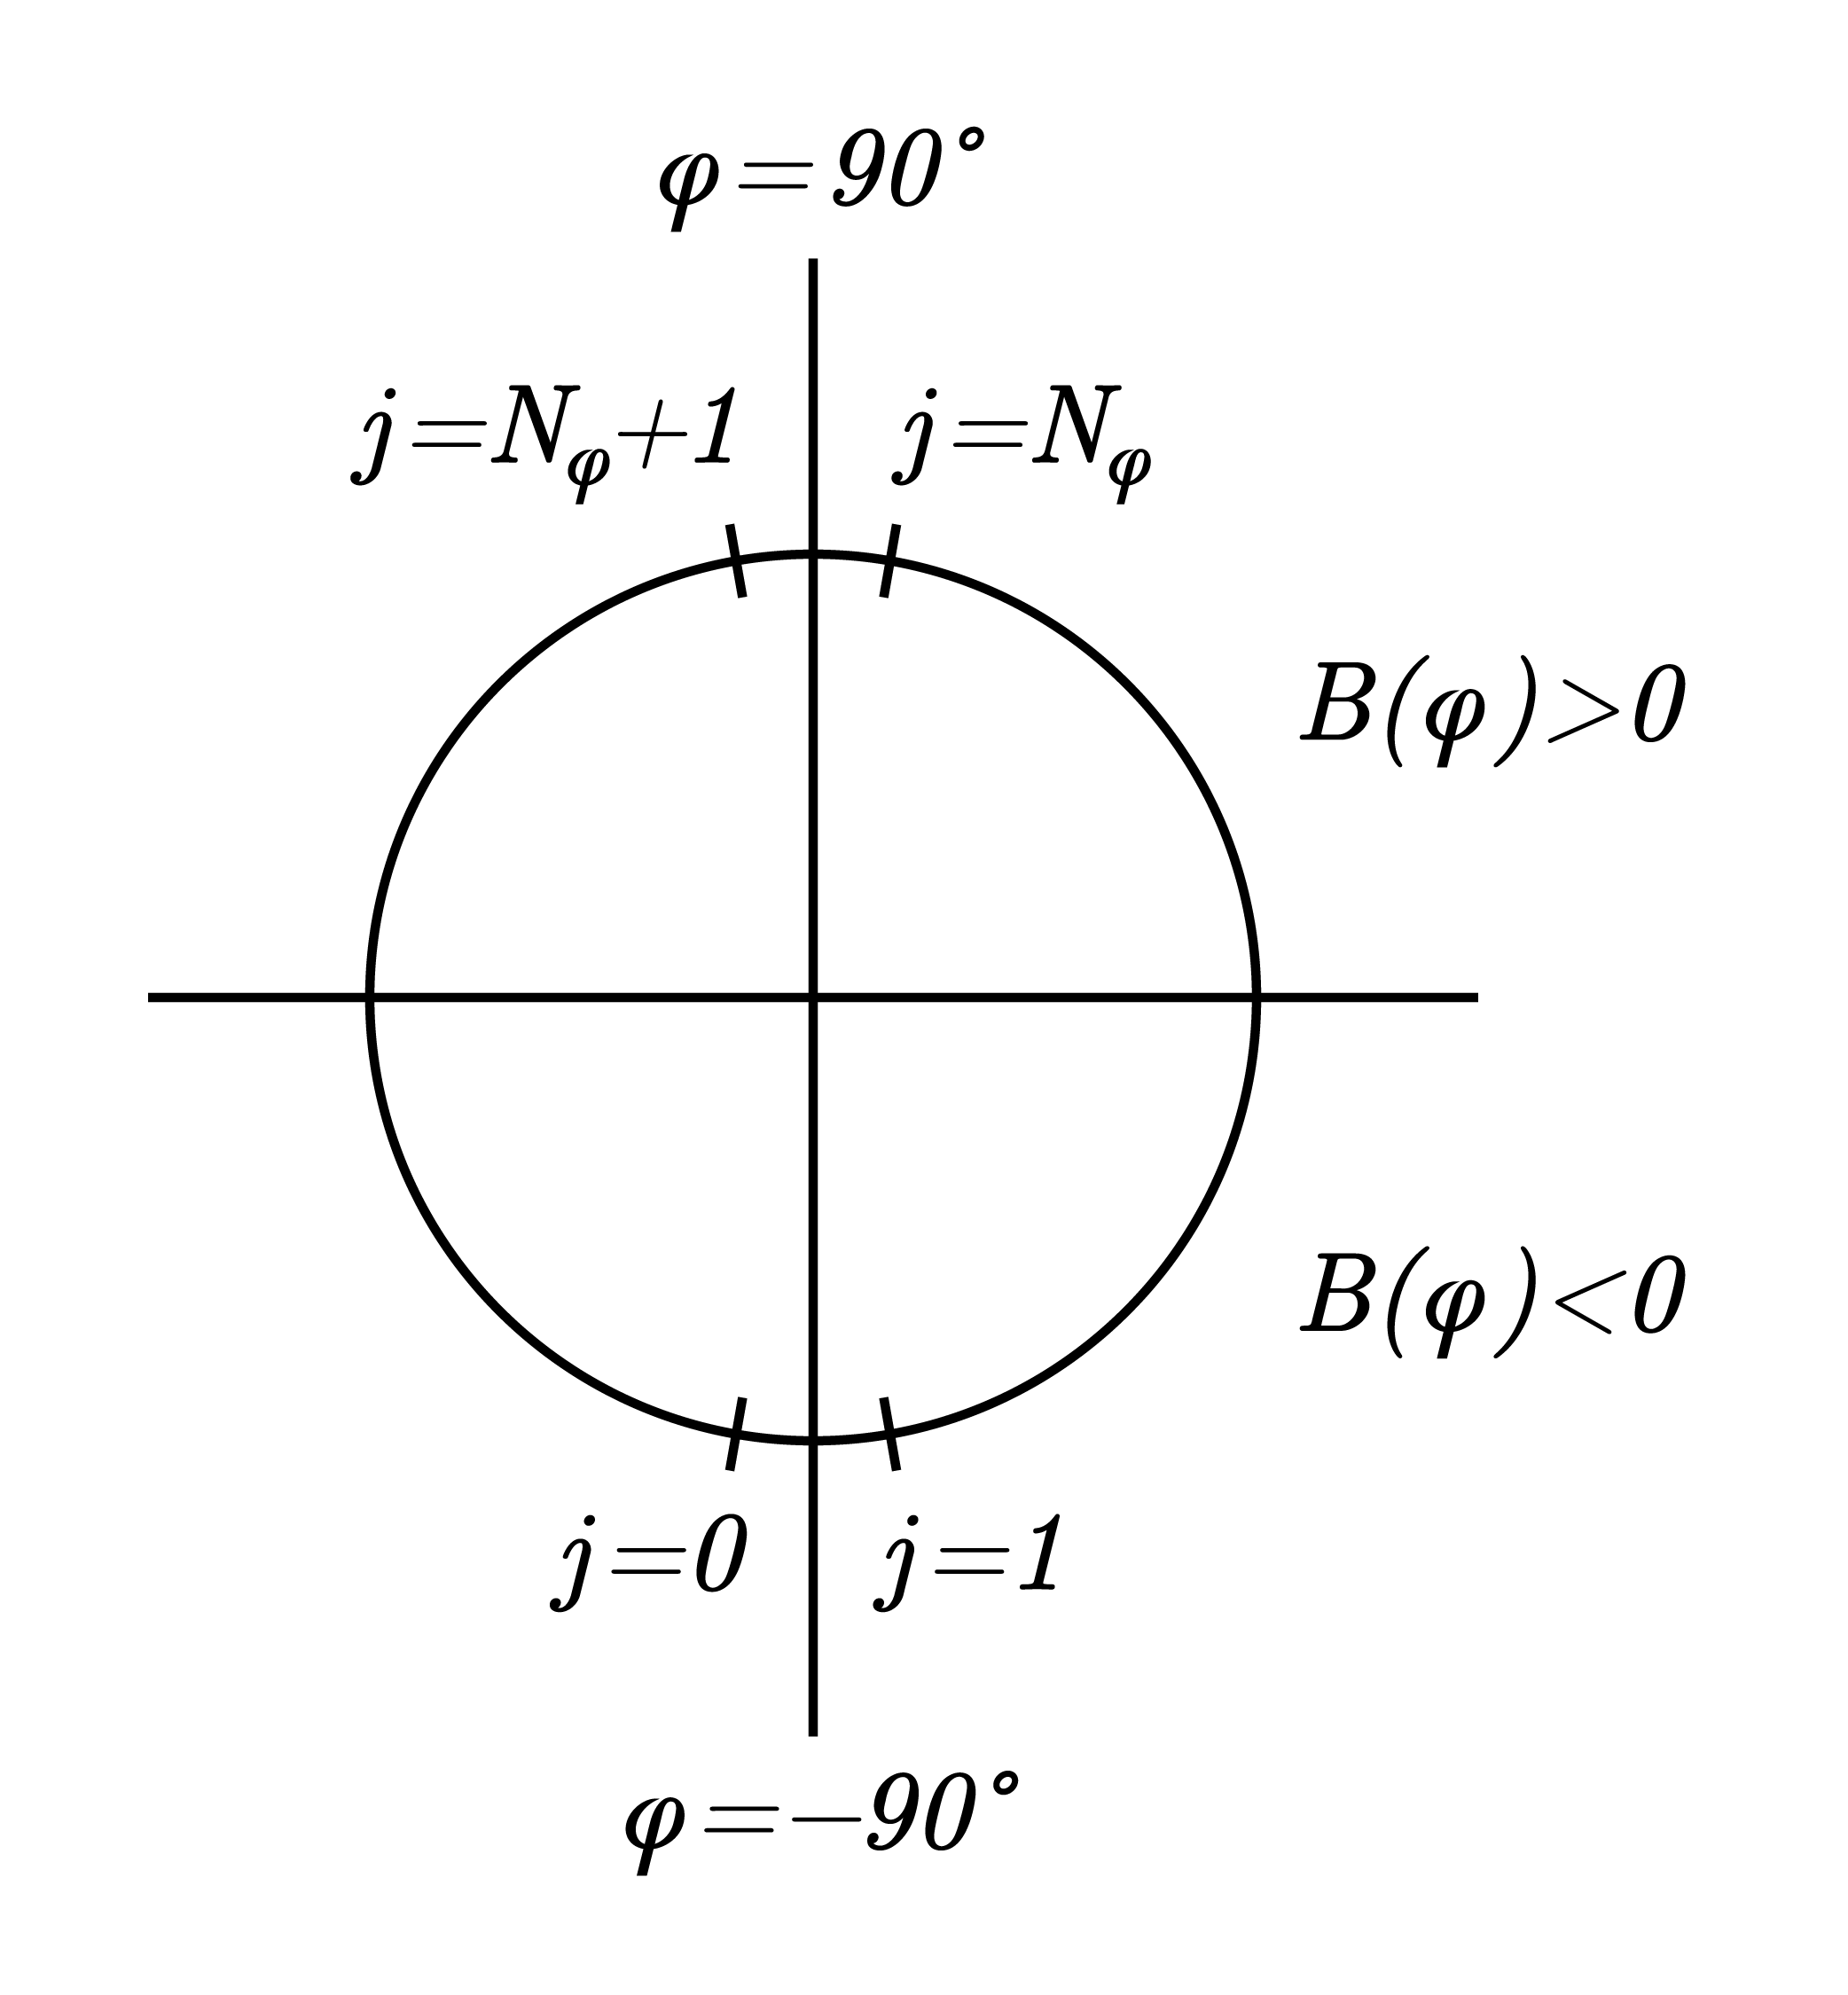
\includegraphics[scale = 0.3]{sphere}
}
\hfill
\parbox[b][5cm][t]{70mm}{

\smallskip

Используются схемы второго порядка аппроксимации, но в окрестности полюсов множитель $\dfrac{1}{\cos\varphi}$ приводит к уменьшению порядка на единицу.

\smallskip

Для вычислений в крайних точках расчетной области отождествляются точки по разные стороны от полюса.

}
\end{frame}



\subsection{Рассматриваемые модели}
\begin{frame}\frametitle{Рассматриваемые модели}

\begin{itemize}
\item[•] Плазмохимия и диффузия вдоль $Oz$: 
$$\dfrac{\partial n}{\partial t} = P-kn+\dfrac{\partial}{\partial z}\left(D\dfrac{\partial n}{\partial z} + \left(\dfrac{1}{T_p}\dfrac{\partial T_p}{\partial z}+\dfrac{1}{H}\right) n\right);$$

\item[•] Полный первый шаг расщепления:
$$\dfrac{\partial n}{\partial t} =P-kn+\dfrac{\partial}{\partial z}\biggl[D\sin^2 I\left(\dfrac{\partial n}{\partial z}+\left(\dfrac{1}{T_p}\dfrac{\partial T_p}{\partial z}+\dfrac{1}{H}\right)n\right)-$$ $$-\dfrac{1}{a}D\sin I\cos I\left(\dfrac{\partial n}{\partial\varphi}+\dfrac{1}{T_p}\dfrac{\partial T_p}{\partial\varphi}n\right)\biggr];$$

\item[•] Двумерная модель: два шага расщепления.
На втором шаге решается уравнение:
$$\dfrac{\partial n}{\partial t} = \dfrac{1}{a\cos\varphi} \dfrac{\partial }{\partial \varphi}\left[\dfrac{D}{a}\cdot(\cos^2  I \cos\varphi)\cdot\dfrac{\partial n}{\partial \varphi} - u\cdot(\sin I \cos I \cos\varphi)\cdot n \right].$$ 
\end{itemize}
\end{frame}


\subsection{Результаты расчетов}
\begin{frame}\frametitle{Результаты расчетов: высотные профили}

Полученные стационарные решения в трёх расссматриваемых моделях при широтах $\varphi = 80^\circ$ и $\varphi = 60^\circ$.

\begin{figure}[H]
\begin{minipage}[c]{0.490\linewidth}
\flushleft
\center{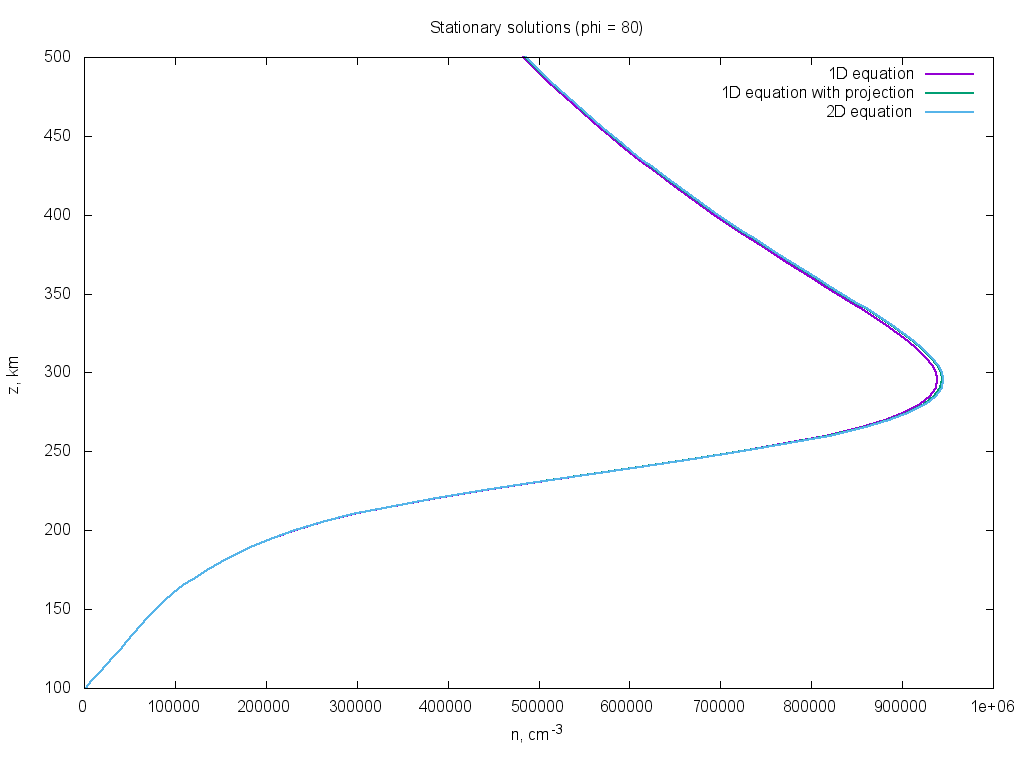
\includegraphics[scale=0.2]{stationary_80}\\$\varphi = 80^\circ$.}
\end{minipage}
\hfill
\begin{minipage}[c]{0.490\linewidth}
\flushleft
\center{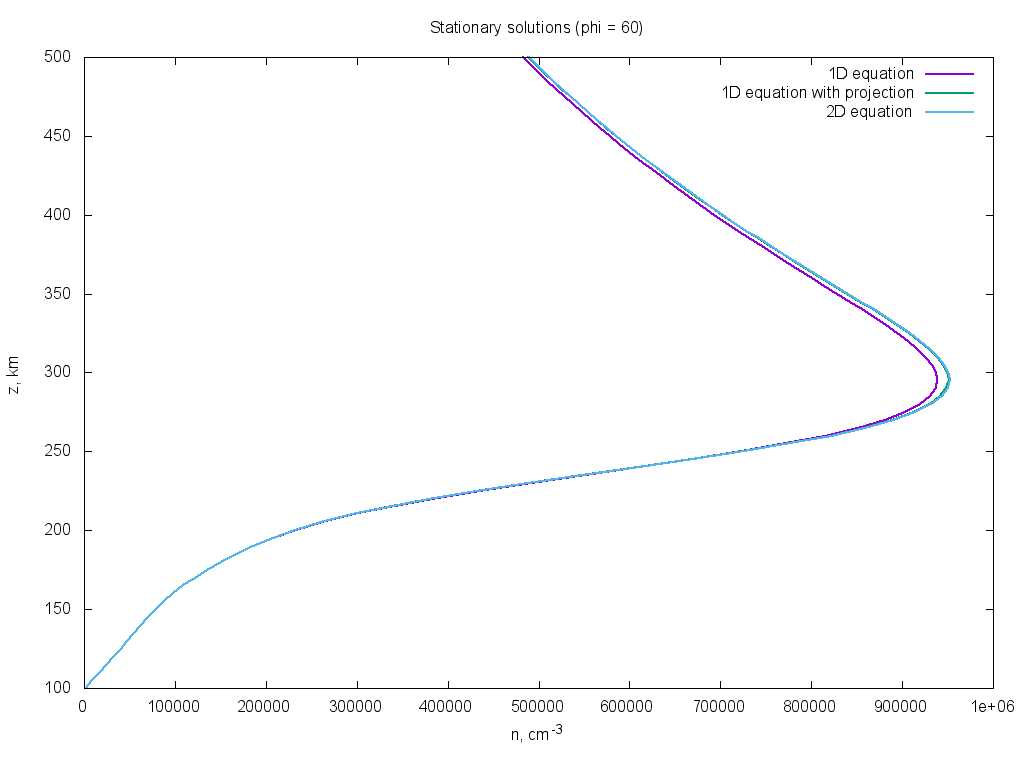
\includegraphics[scale=0.2]{stationary_60}\\$\varphi = 60^\circ$.}
\end{minipage}
\end{figure}

\end{frame}

\subsection{Результаты расчетов}
\begin{frame}\frametitle{Результаты расчетов: высотные профили}

Полученные стационарные решения в трёх расссматриваемых моделях при широтах $\varphi = 2^\circ$ и $\varphi = 1^\circ$.

\begin{figure}[H]
\begin{minipage}[c]{0.490\linewidth}
\flushleft
\center{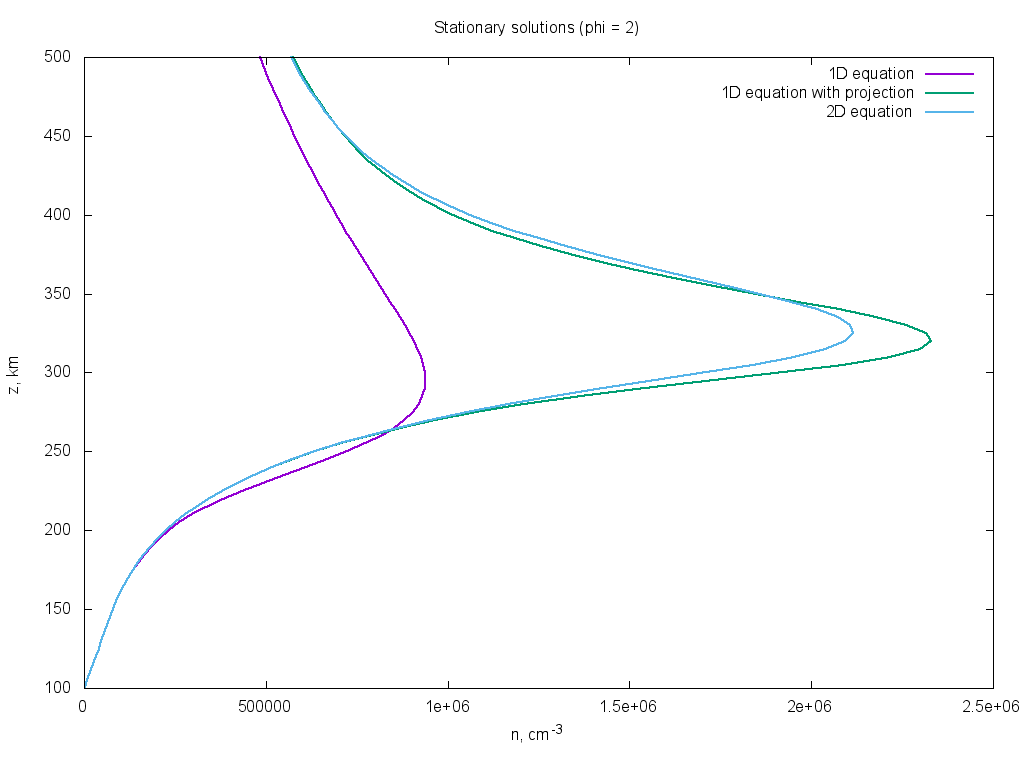
\includegraphics[scale=0.2]{stationary_2}\\$\varphi = 2^\circ$.}
\end{minipage}
\hfill
\begin{minipage}[c]{0.490\linewidth}
\flushleft
\center{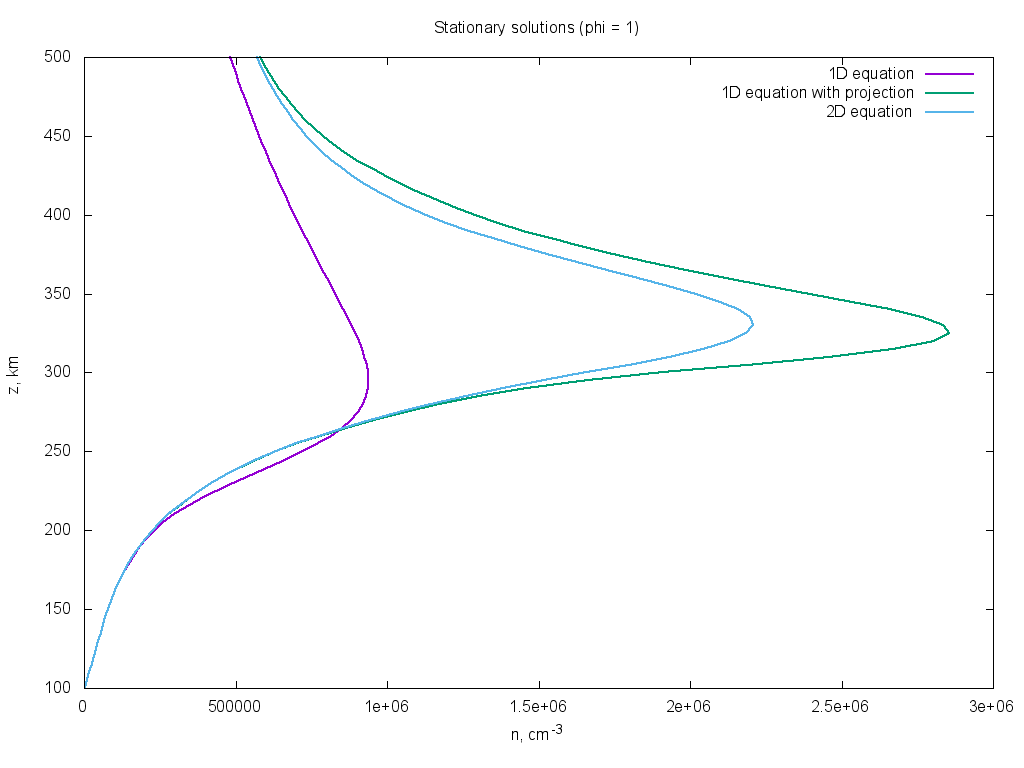
\includegraphics[scale=0.2]{stationary_1}\\$\varphi = 1^\circ$.}
\end{minipage}
\end{figure}

\end{frame}

\subsection{Результаты расчетов}
\begin{frame}\frametitle{Результаты расчетов}

Стационарные решения при расчетах в соответствии с одним или двумя шагами расщепления.

\begin{figure}[H]
\begin{minipage}[c]{0.490\linewidth}
\flushleft
\center{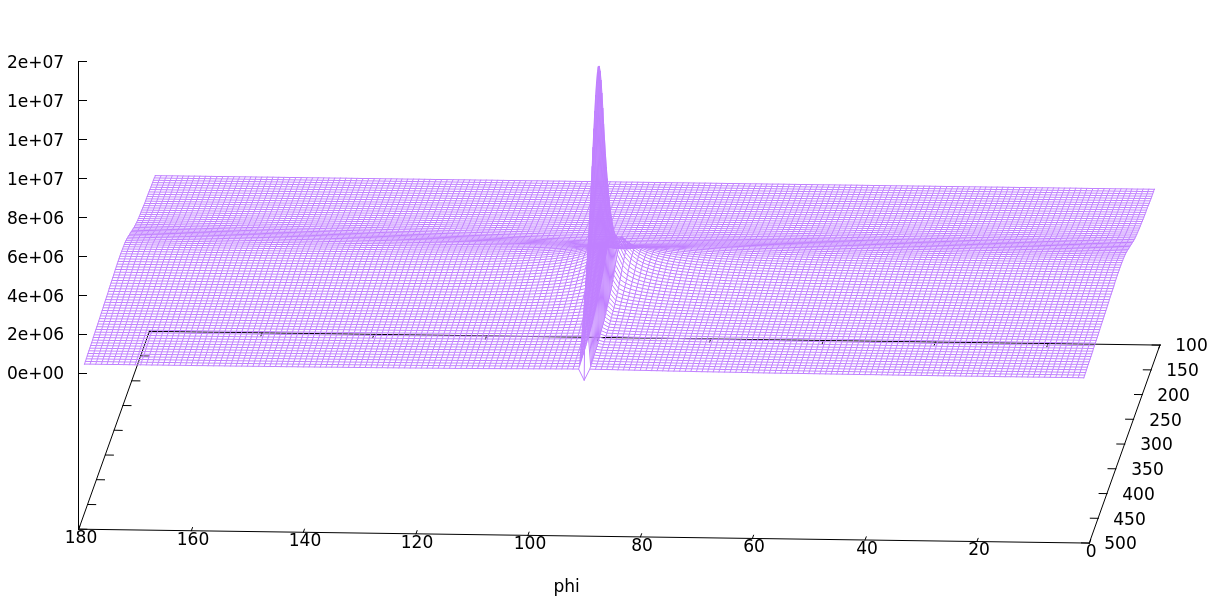
\includegraphics[scale=0.145]{step1}\\Первый шаг расщепления.}
\end{minipage}
\hfill
\begin{minipage}[c]{0.490\linewidth}
\flushleft
\center{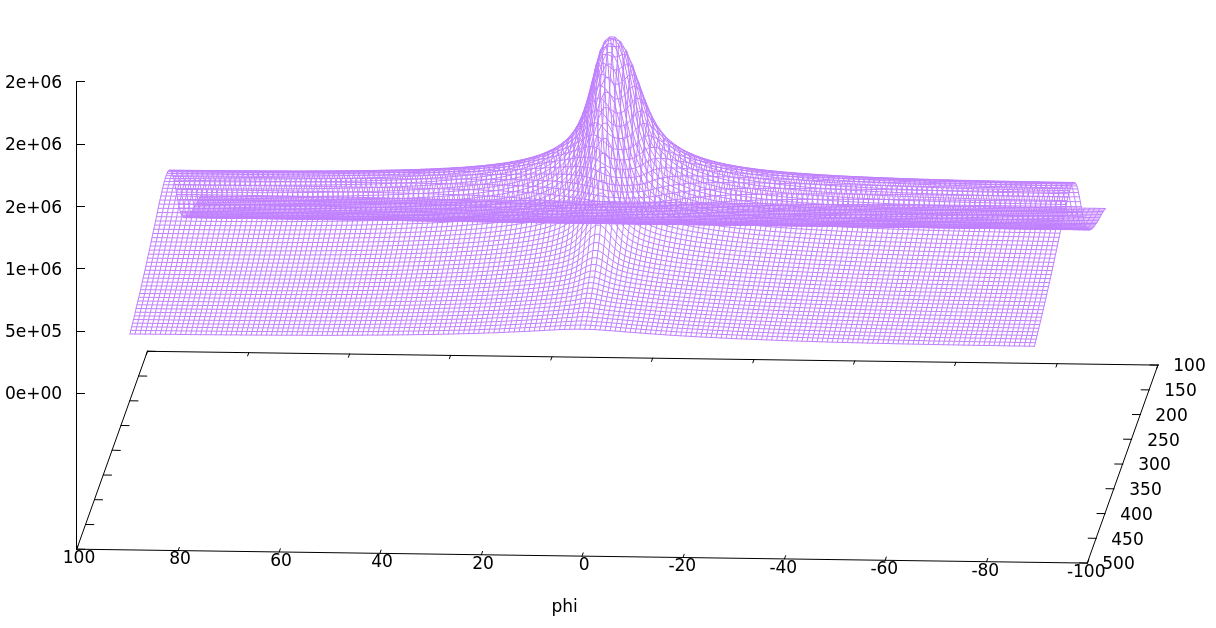
\includegraphics[scale=0.145]{step2}\\Два шага расщепления.}
\end{minipage}
\end{figure}


\end{frame}




\begin{frame}[plain]
  \begin{center}
  {\Huge Спасибо за внимание!}
  \end{center}
\end{frame}


\subsection{Приложение 1: входящие в уравнение параметры}
\begin{frame}\frametitle{Приложение: входящие в уравнение параметры}
Для функций $P$, $k$, температур и концентраций $N_2$, $O_2$ и $O$ используются аналитические формулы: 

\begin{itemize}
\item[•] $T(z)=T_\infty - (T_\infty-T_0)\exp\left(-\dfrac{g}{RT_\infty}(z-z_0)\right),$ 

$T_{n\infty}=800$~К, $T_{i\infty}=950$~К, $T_{e\infty}=2200$~К.

\smallskip

\item[•] Для концентраций~---~Больцмановское распределение: $n_{O_2, N_2, O} (z)= n_{O_2, N_2, O} (z_0)\cdot \exp\left(-\dfrac{M_{O_2, N_2, O}g}{R_0T_n}(z-z_0)\right).$ 

На высоте $100$~км $n_{O_2} = 5{,}6\cdot 10^9$~см$^{-3}$, $n_{O} = 2{,}8\cdot 10^{10}$~см$^{-3}$, $n_{N_2} = 5{,}2\cdot 10^{10}$~см$^{-3}$.

\smallskip


\item[•] В дневное время $P=4\cdot10^{-7}n_O(z)$;

$k=1{,}2\cdot10^{-12}n_{N_2}(z)+2{,}1\cdot10^{-11}n_{O_2}(z)$
\end{itemize}

\end{frame}

\subsection{Приложение 2: коэффициенты в уравнении второго шага}
\begin{frame}\frametitle{Приложение: коэффициенты в уравнении второго шага}

Рассмотрим функции: $$A(\varphi) = \dfrac{\cos\varphi}{1+4\tg^2\varphi}\mbox{ и }B(\varphi) = \dfrac{4\sin\varphi}{1+4\tg^2\varphi}.$$

Имеют место следующие разложения при $\varphi\rightarrow\dfrac{\pi}{2}$: $$A(\varphi)=-\dfrac{1}{4}\cdot\left(\varphi-\dfrac{\pi}{2}\right)^3+o\left(\left(\varphi-\dfrac{\pi}{2}\right)^5\right); B(\varphi) = 1\cdot\left(\varphi-\dfrac{\pi}{2}\right)^2+o\left(\left(\varphi-\dfrac{\pi}{2}\right)^4\right)$$

Аналогичные асимптотики и при $\varphi\rightarrow - \dfrac{\pi}{2}$



Графики функций $A$ и $B$ приведены ниже: 
\parbox[b][3cm][t]{60mm}{
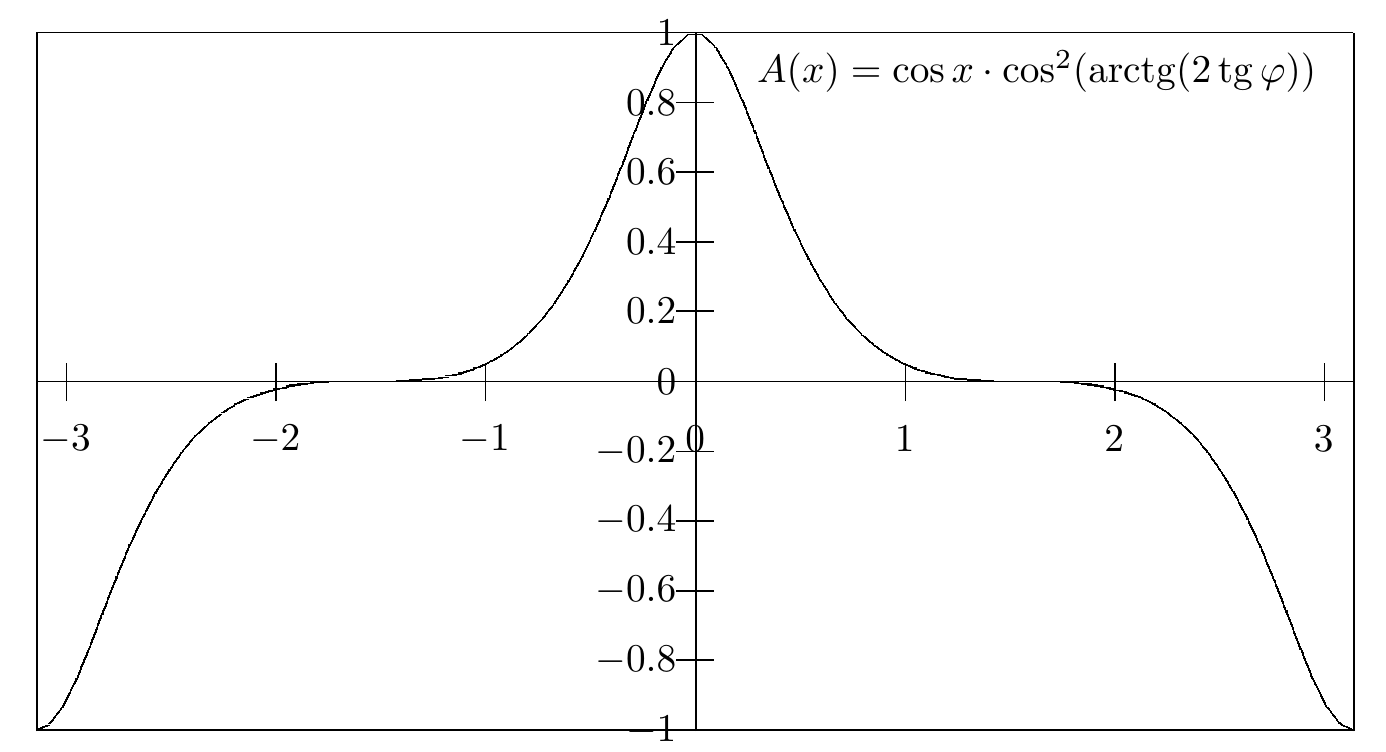
\includegraphics[scale=0.12]{A}}
\hfill
\parbox[b][3cm][t]{60mm}{
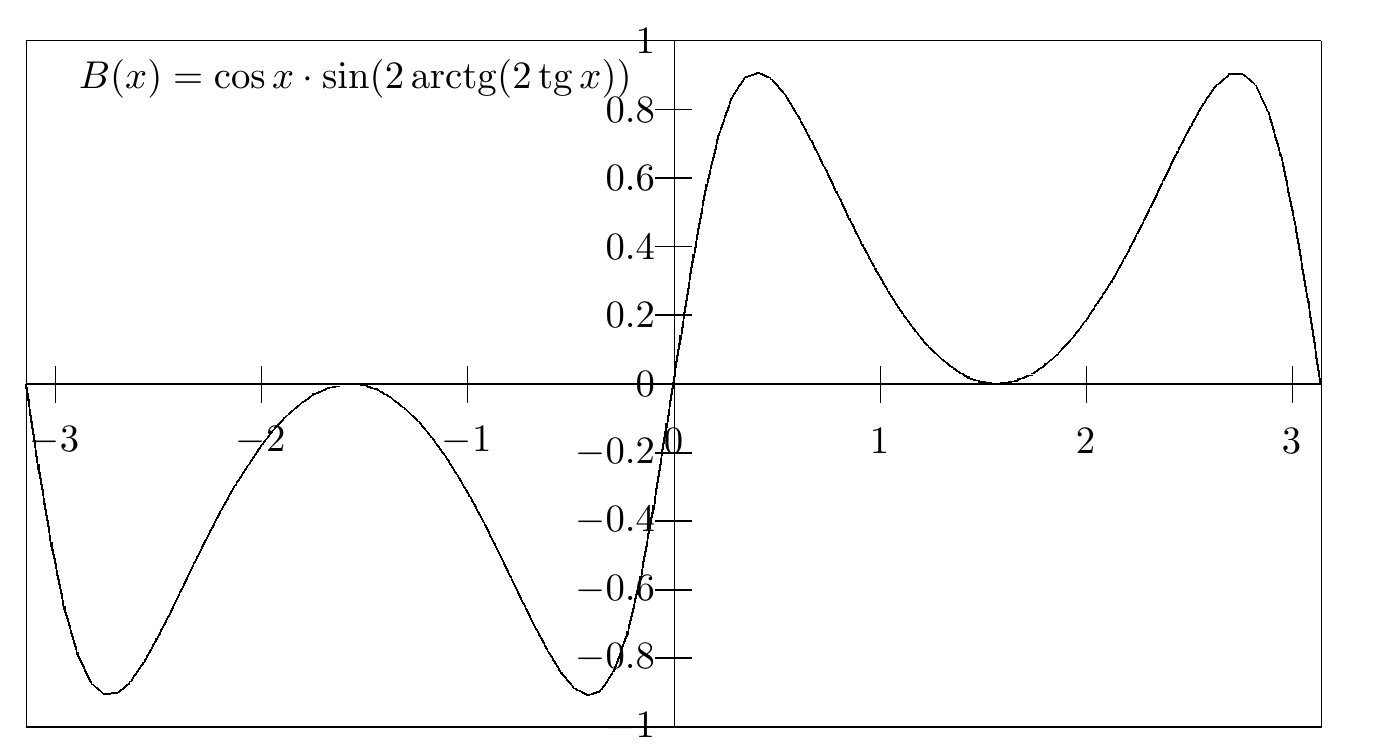
\includegraphics[scale=0.12]{B}}


\end{frame}


\end{document}
